\documentclass{article}

\usepackage{graphicx} % Required for inserting images
\usepackage[utf8]{inputenc}
\usepackage{fvextra}
\usepackage{csquotes}
\usepackage[backend=biber,style=apa]{biblatex}
\usepackage[a4paper, total={6.25in, 9in}]{geometry}
\usepackage{tikz}
\usepackage{booktabs}
\usepackage{multirow}
\usepackage{scalerel}
\usepackage[toc,page]{appendix}
\usepackage{minted}
\usepackage{geometry}
\usepackage[T1]{fontenc}
\usepackage[english]{babel}
\usepackage{xcolor}
\usepackage{subcaption}
\usepackage{listings}
\usepackage{titling}

\def\checkmark{\tikz\fill[scale=0.4](0,.35) -- (.25,0) -- (1,.7) -- (.25,.15) -- cycle;}
\addbibresource{references.bib}

\newcommand{\mysubtitle}[1]{\posttitle{\par\end{center}\begin{center}\large#1\end{center}\vskip0.5em}}

\title{Exploring OpenAI's GPT Model in Political Context}
\mysubtitle{A New Type of Dataset for Political Science Research}


\author{
  Laurence-Olivier M. Foisy
  \and
  Hubert Cadieux
  \and
  Étienne Proulx
  \and
 Jérémy Gilbert
  \and
  Jozef Rivest
  \and
  Alexandre Bouillon
  \and
  Yannick Dufresne
}

\date{\today}

\begin{document}

\maketitle

\begin{abstract}
   This research note shares a new type of dataset that could provide insights into potential algorithmic biases contained within OpenAI's GPT model. This contribution is important in a context where large language models, and ChatGPT in particular, could become widely-used heuristic tools for accessing political information. The dataset was generated by using OpenAI's API to prompt a GPT model about the key characteristics of every member of the 43rd Canadian parliaments and the 42nd National Assembly of Quebec. Next, a clustering tool was used to extract the themes of each politician's characteristics. Descriptive statistic methods then revealed differences in themes used to describe politicians of different parties, genders, and regions, raising questions about potential algorithmic biases. Sharing datasets like this one and providing researchers with the methods to acquire new ones could help forage deeper into the understanding of large language models' algorithmic biases and the implications of using these new tools in shaping the political landscape. 
\end{abstract}

\section{Introducing a New Type of Dataset}

This research note presents a new type of dataset compiled by prompting ChatGPT, a large language model (LLM) developed by OpenAI and launched on November 28, 2022. Data from ChatGPT is of great interest to political science research given its recent emergence and immediate widespread popularity. However, as a proprietary model, the origin of the information and the parameters that make up ChatGPT are unknown, which raises questions about the provenance of the training data used by OpenAI. The opacity of the model makes it difficult to understand its inner workings, which limits users' ability to assess the reliability of the answers provided. In a context where LLMs, particularly ChatGPT, are widely employed by the general public to access information on crucial topics like politics, conducting thorough research to comprehend the implications of their usage and identify potential bias risks becomes imperative. That is why it is important to explore innovative data collection methods to allow the scientific community to push the research further.

The dataset presented in this research note has the potential to enable the analysis of algorithmic biases that may emerge from the use of ChatGPT. Hartman identifies three possible biases: majority biases from training datasets containing unbalanced human-biased information, biases coming from human implication in the training procedure, and biases coming from human-set guardrails preventing the model from generating harmful content.\parencite{hartmann_etal23}. Additionally, according to the ecological rationality theory, LLMs have the potential to become widespread heuristic tools for their ability to be time-saving, and because they can provide concise information about parties and candidates. Hence, the presence of biases in these tools is problematic as it may raise issues about the degradation of democracy, which relies on free, and diversified sources of information to operate optimally \parencite{dahl06}. This is especially alarming as we are witnessing rapid growth in widely available artificial intelligence systems and as our reliance on these systems increases. \parencite{rozado23} However, the main contribution of this shorter note is not to determine whether biases are present or not but to begin the necessary work of extracting data from a closed, opaque source and make it open source for the scientific community to access and push research further. This dataset is related to political science but the methods used to assemble it could very well be applied to any other field of social science.\par

\section{VAAs as Digital Heuristic Tools}

In a complex environment like the ecosystem of an election, most voters are likely not cognitively and knowledgeably competent enough to make decisions based on complex methods. As a result, humans are prone to take shortcuts, also known as heuristics, while making these decisions, thus ignoring parts of the available information \parencite{gigerenzer_gaissmaier11}. \par

In recent years, the emergence of new technologies has allowed citizens to use new digital tools as heuristics in election contexts. These new heuristics tools\footnote{ Neth and Gigerenzer define heuristics as "adaptative tools that ignore information to make fast and frugal decisions that are accurate and robust under conditions of uncertainty" \parencite{neth_gigerenzer15}} are developed to help citizens make their vote choice. Among these tools, the \textit{voting advice applications} (VAA) are increasingly popular and have been tested in a multitude of contexts \parencite{garzia_marschall12, garzia_marschall19}. These tools require a great amount of attention from the political science community considering their significant effect on voters' turnout and vote choice in electoral contexts.

\textit{Turnout.} A strand in the VAAs' literature is interested in how much these applications can affect the electoral participation \parencite{germann_gemenis19, stadelmann-steffen_etal22}. Even if there's no consensus on the effect these tools have on turnout, some research has demonstrated that they can boost electoral participation, especially by mobilizing groups that tend to vote in small numbers like young voters and politically less knowledgeable voters \parencite{gemenis_rosema14}.

\textit{Vote choice.} Some studies have shown that VAAs can have a substantial effect on voters' decisions, especially among people with a \textit{moderate level of interest} in politics \parencite{tromborg_albertsen23}. Others have demonstrated that these tools can engage voters in policies by "providing insights into public opinion by assessing respondents' views on different policy questions" \parencite{lees-marshment_etal15}. For example, in the 2014 national election in New Zealand, 330,000 people, over 13\% of voters, used the electoral compass, a VAA, to assist them in their decision-making process. It thus seems evident that these tools could play a role in favoring parties over others in the aggregate results of an election. Thus, because of their potential effect and their accessibility, it is important to understand how these tools work and how they provide information to voters.

\section{LLMs as New VAAs}
The recent emergence of LLM chatbots such as ChatGPT has the potential to considerably affect the world of heuristic tools by providing new and efficient ways to make fast and frugal decisions in electoral contexts \parencite{kim_lee23}. Based on the \textit{ecological rationality} theory, voters tend to employ heuristics that satisfy three key criteria: (1) low information costs, (2) ease of use, and (3) improved average accuracy. \parencite{tromborg_albertsen23}. Thus, LLMs could represent new significant tools for voters to maximize these three criteria in the near future. Rationally, they are an efficient and time-saving instrument that could help voters review parties' positions on salient issues, and learn about each party's candidates or leaders. This information can then be used by voters to make their decision. \par

However, too little is known about the training of LLMs and how they generate information about political parties and candidates. It is imperative to address this lack of knowledge and the questions that arise from this unknown. In the literature on VAAs, some have raised questions about the accountability of researchers who develop VAAs \parencite{ladner_etal10, romeromoreno_etal22}. These normative questions are especially important considering the effect VAAs can have on voting behaviours and election turnout. While it is easier to retrace the methodology used in VAAs, as many articles do by criticizing some core aspect of their modeling algorithms \parencite{vanderlinden_dufresne17, louwerse_rosema14, romeromoreno_etal22}, LLMs and AI models are less transparent in the way they work and are prone to biases, and hallucinations, defined as "confident responses that seemed faithful [but that are] non-sensical when viewed in light of the common knowledge in these areas." \parencite{alkaissi_mcfarlane23} So, given the increasing popularity of LLMs and the gap to be filled in the study of LLMs as heuristics, ChatGPT becomes an excellent study case as it has the potential to help voters acquire information and make decisions \parencite{hartmann_etal23}. It is therefore necessary to assemble datasets and measurement tools to measure the algorithmic biases of LLMs.\par

Some have already demonstrated that ChatGPT had a "pro-environmental, left-libertarian orientation" aligned to more liberal, educated, and wealthy people \parencite{hartmann_etal23, santurkar_etal23, rutinowski_etal23, kim_lee23}. These studies open up the discussion about the social impact of chatbots. Especially on how they could potentially affect voting behaviours, participation, and turnout by providing biased information to users. \par

The main goal of this note is to introduce new ways to create innovative electoral studies datasets using the OpenAI API to open up the study of LLM algorithmic biases.

\section{Dataset}

We provide a dataset containing the following variables :

\begin{table}[h]
\centering
\caption{Dataset description}
\begin{tabular}{@{}p{4cm}cc@{}}
\toprule
Variable                                 & Quebec provincial ridings & Canadian federal ridings \\
\midrule
MP/MNA's names                       & \checkmark & \checkmark \\
MP/MNA's Party                         & \checkmark & \checkmark \\
Legislature                              & \checkmark & \checkmark \\
Riding's name                            & \checkmark & \checkmark \\
Riding's id number                       & \checkmark & \\
Riding's province                        &            & \checkmark \\
\midrule
2016 census data of SES variables in the ridings: &  &  \\
\quad Gender                             & \checkmark & \\
\quad Age                                & \checkmark & \\
\quad Language spoken                    & \checkmark & \\
\quad Income level                       & \checkmark & \\
\quad Education level                    & \checkmark & \\
\midrule
Riding vote shares in the 2018 election   & \checkmark & \\
MP/MNA's 10 characteristics given by ChatGPT & \checkmark & \checkmark \\
Theme (as generated by Novacene AI clustering) & \checkmark & \checkmark \\
Wikidata QID of the MP/MNA                   & \checkmark & \checkmark \\
MP/MNA's Gender                         & \checkmark & \checkmark \\
\bottomrule
\end{tabular}
\end{table}


\subsection{Prompting ChatGPT Multiple Times}
We initiated the process by compiling a list of all 338 + 2 Members of Parliament (MPs) serving in the 43rd Canadian House of Commons and 125 Members of the National Assembly (MNAs) serving in the 42nd National Assembly of Quebec.\footnote{There are 338 seats in the House of Commons of Canada but 340 MPs entries in the dataset due to changes during the legislature.} This list was assembled using publicly accessible information and included MPs/MNA's respective electoral ridings.

Next, we used the \textit{openai} package in Python to prompt GPT's \textit{text-davinci-003} model.\footnote{After trying a various array of models (babbage, curie, davinci, and gpt-3.5-turbo), we chose to use the text-davinci-003 model. It reacted efficiently and reliably to the different prompts we tested and allowed us to conveniently format the outputs in a way that made it easy to include them in the dataset.} After testing multiple prompts, we settled on the following:

\begin{quote}
    \textit{Provide a list of 10 key characteristics describing [Canada/Quebec] MP [MP's name]'s policies formatted in a .csv style output, all on the same line. (ex: MP name, Characteristic 1, characteristic 2, characteristic 3, characteristic 4, characteristic 5, characteristic 6, characteristic 7, characteristic 8, characteristic 9, characteristic 10)}
\end{quote}

We decided to deliberately omit to mention the politicans' party as this could have enabled the model to fill in the gaps in cases where it lacked information about candidates and generate content based on the MP/MNA's party affiliation rather than relying solely on the provided name. Appendix \ref{appendix:codesnippet} contains the snippet of code that was used to generate these data.

OpenAI's API access pricing was negligible in generating the dataset. We paid \$0.0200 / 1K tokens inputs and outputs.\footnote{LLMs way of dealing with words and sentences is to decompose them into Tokens through a process called Tokenization.\parencite{maeda_bolanos23} Researchers can preview how many tokens an input string will be equivalent to by using OpenAI's Tokenizer tool at: https://platform.openai.com/tokenizer} Including the testing of different prompts, different models, and different temperatures, as well as the generation of the actual dataset, the total price ended up under USD \$2.50.

\subsection{Enriching our Dataset}

To conduct comprehensive descriptive analyses of our dataset, we enriched it by integrating information from various additional data sources.

The first step of enriching our data was to assign a general theme to each value returned by OpenAI's model. This simplified the process of describing the dataset. To accomplish this, we used the NovaceneAI \parencite{novaceneaiplatformtm23} platform for automated textual analysis, which allowed us to conduct clustering analysis and extract the general theme of each characteristic of the MP/MNAs. Manual validation on a subset of the data was then carried out and some observations were manually corrected. The themes generated by the NovaceneAI Platform™ as well as the original characteristics returned by OpenAI's model are included in the dataset provided in this shorter note.\footnote{We employed NovaceneAI's tools for clustering in our research due to their offer of platform access, which allowed us to explore its capabilities. The outcomes obtained from the clustering process proved to be satisfactory so we decided to integrate them into our analysis. Since our project's  goal is to democratize access to private closed-source data, the decision to use a clustering algorithm from a private company may seem paradoxical. However, we chose this methodological approach to simplify and streamline the aggregated description of the data. As mentioned in the note, the original characteristics returned by OpenAI's model are present in the provided dataset and thus available for researchers wanting to conduct textual analysis with their own tools.}

We integrated additional relevant variables to our dataset such as gender (fetched through the Wikidata API),  MP's riding vote shares in the 2018 Quebec general election (for Quebec provincial ridings only), and the 2016 census data for the MP's riding (for Quebec provincial ridings only). All these variables combined made for an innovative dataset, ready to be used for bias analysis.

\subsection{Descriptive Statistics}

\subsubsection{By Party}

The left-hand portion of \textit{Figure \ref{byparty}} represents the themes most mobilized by ChatGPT to describe MPs from federal parties. The portion on the right represents the same for Quebec provincial MNAs. We can see that the 5 themes most mobilized by ChatGPT for both the federal and provincial parties are the same at slightly different proportions. Those five important themes are: \textit{social justice}, \textit{economic development}, \textit{environment}, \textit{fiscality} and \textit{health}. \par
Also, the proportional distribution of themes used by ChatGPT is similar from party to party. However, some parties stand out from others. For example, among the federal parties, \textit{social justice} comes up less often for the Conservative Party of Canada (CPC), at 13.63\%, than other parties. It can be noted that, for the \textit{environment} theme at the federal level, the GPC stands out from other parties with a proportion of 40\%. However, it is interesting to note that ChatGPT uses the \textit{economic development} theme to a lesser extent for the GPC (5\%) than for other parties. In addition, the CPC stands out from the other parties for its mentions of the \textit{fiscality} theme, with a proportion of 16\%. \par
At the provincial level, the Coalition Avenir Québec (CAQ) and the Parti Québécois (PQ) stand from the other parties for the theme of the \textit{environment}, with proportions of 29.34\% and 31.25\% respectively. On the other hand, Québec Solidaire (QS) stands out from others with its high proportion of the \textit{social justice} theme at 31.96\%, as described by ChatGPT. 

\begin{figure}[H]
\centering
\vstretch{1}{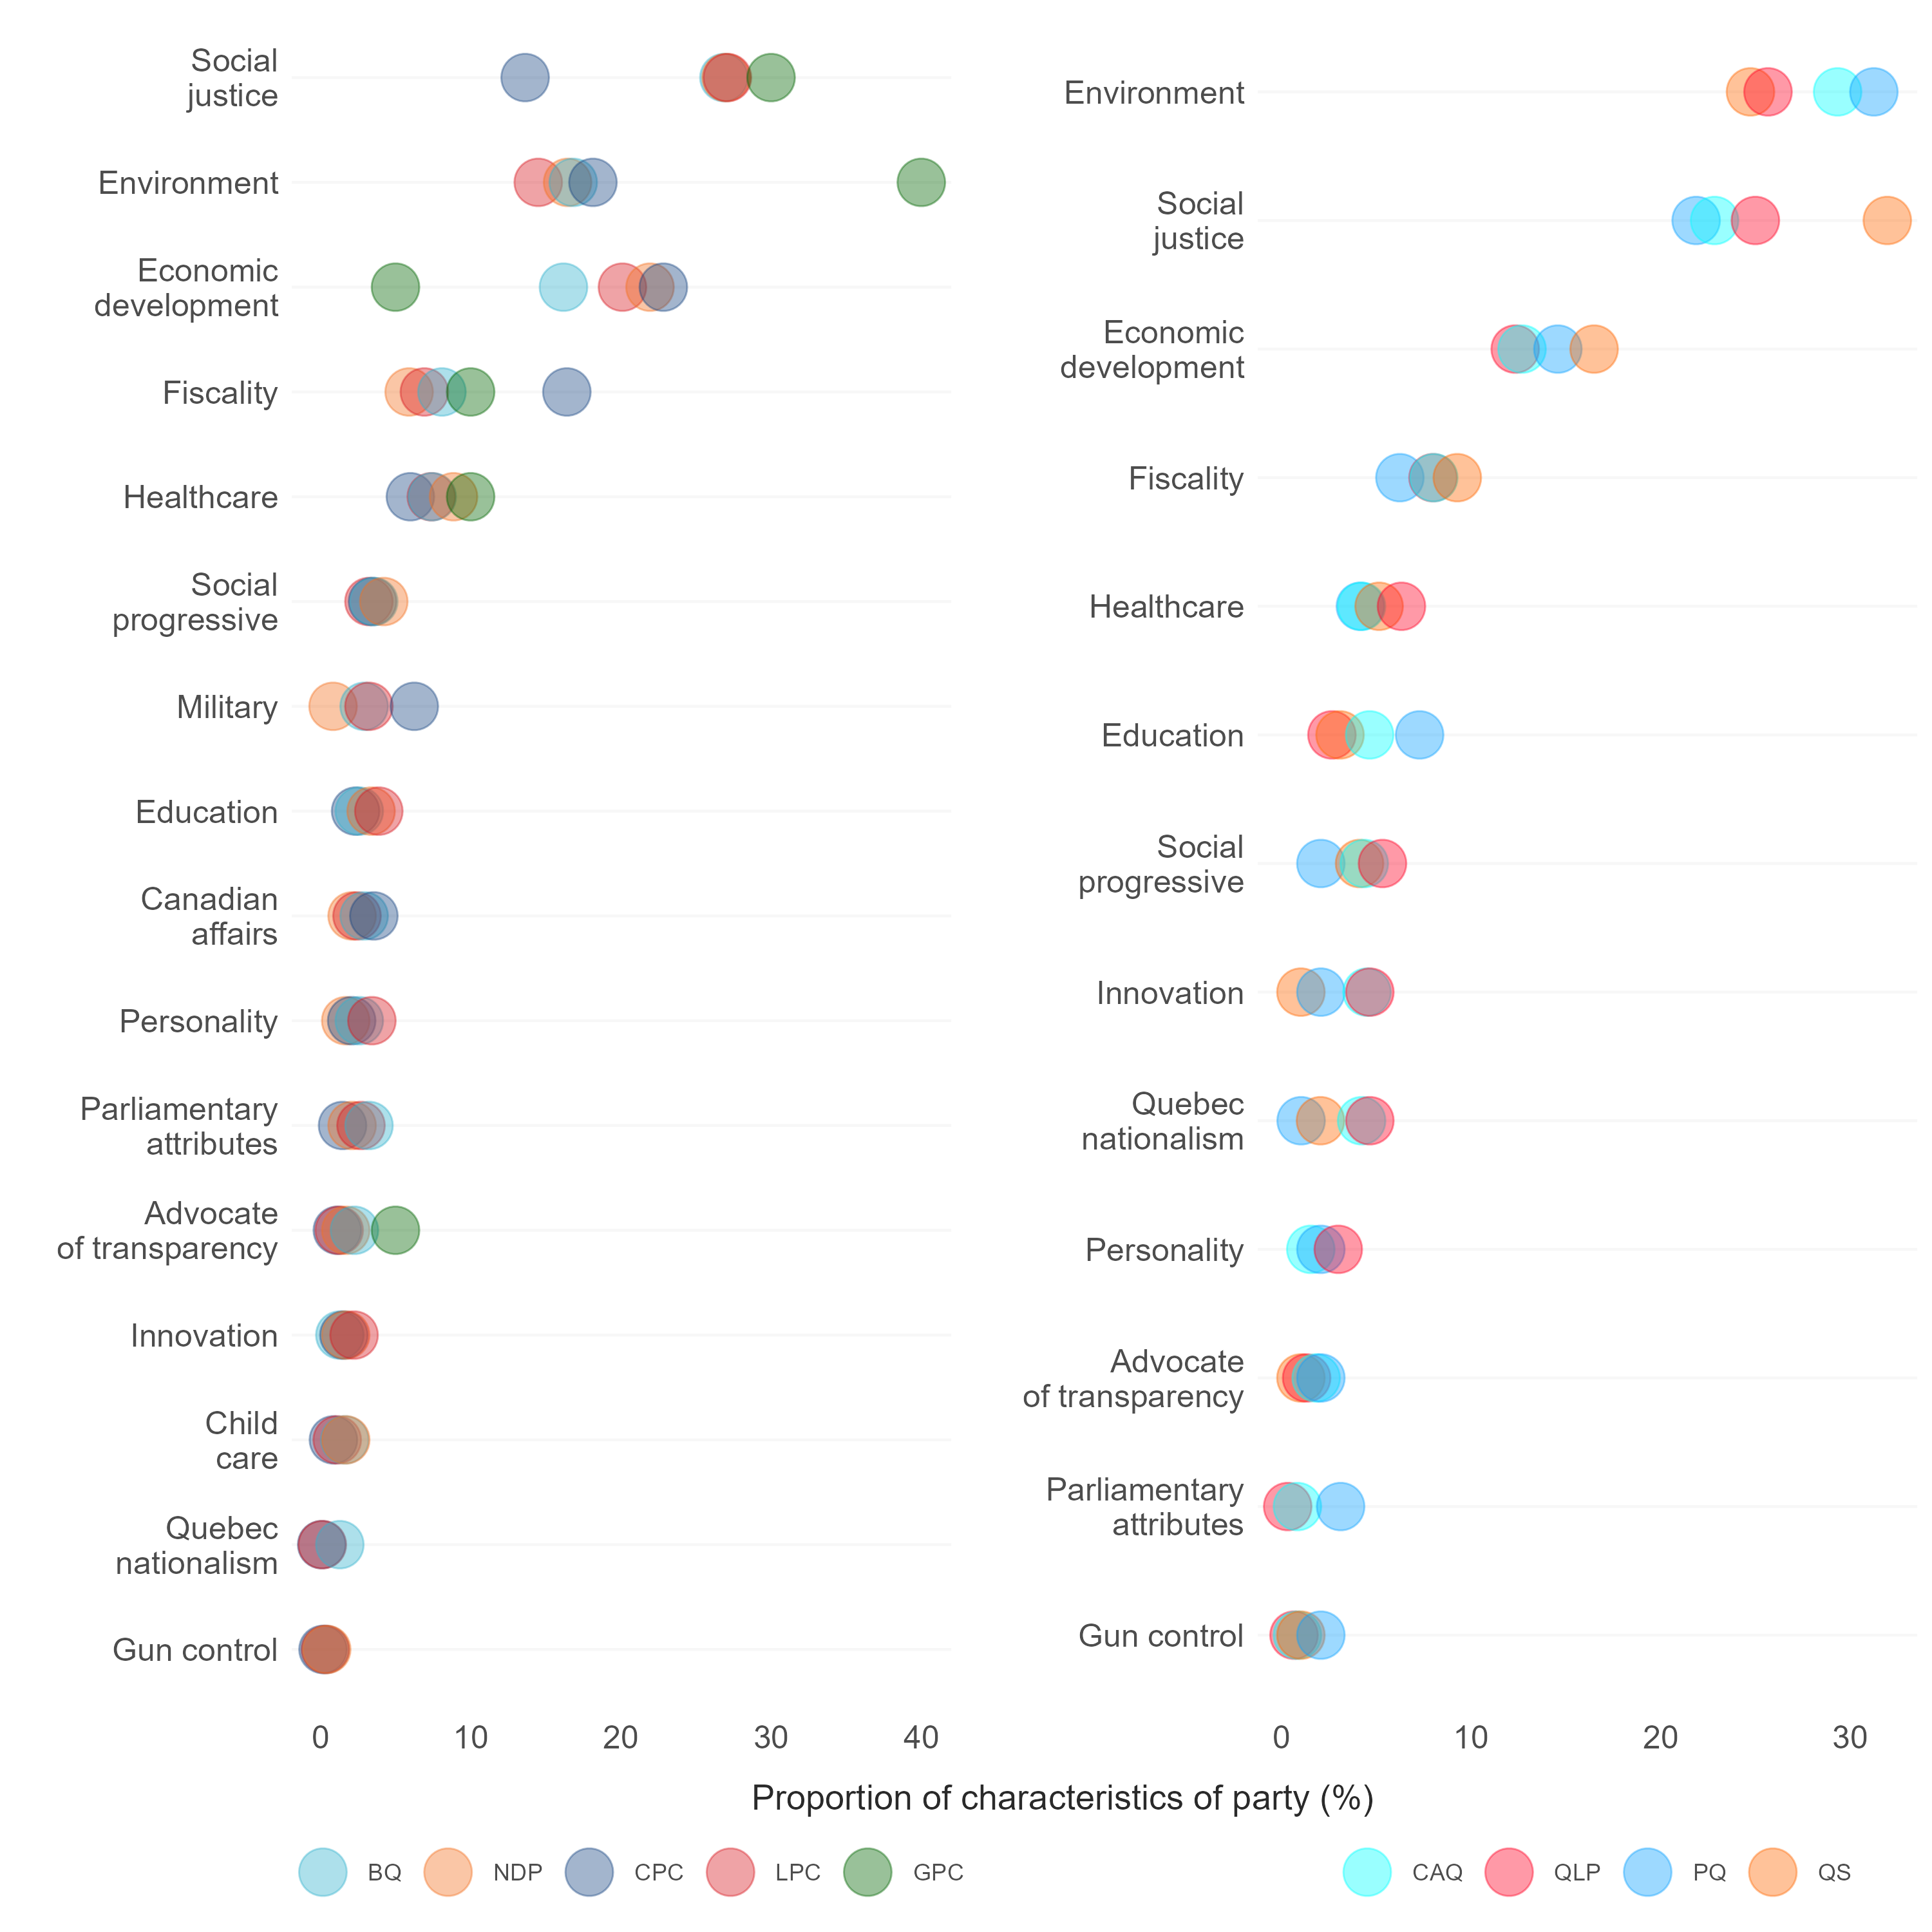
\includegraphics[scale = 0.5]{by_party.png}}
\caption{Analysis of \textit{davinci-003} Model's Most Used Characteristic Issues by Political Party}
\begin{minipage}{0.7\textwidth}
\footnotesize \textit{Note}: Theme labeling is derived from the Novacene AI clustering algorithm.
\label{byparty}
\end{minipage}
\end{figure}

\subsubsection{By Gender}

\begin{figure}[H]
    \centering

    \begin{subfigure}[b]{0.45\textwidth}
        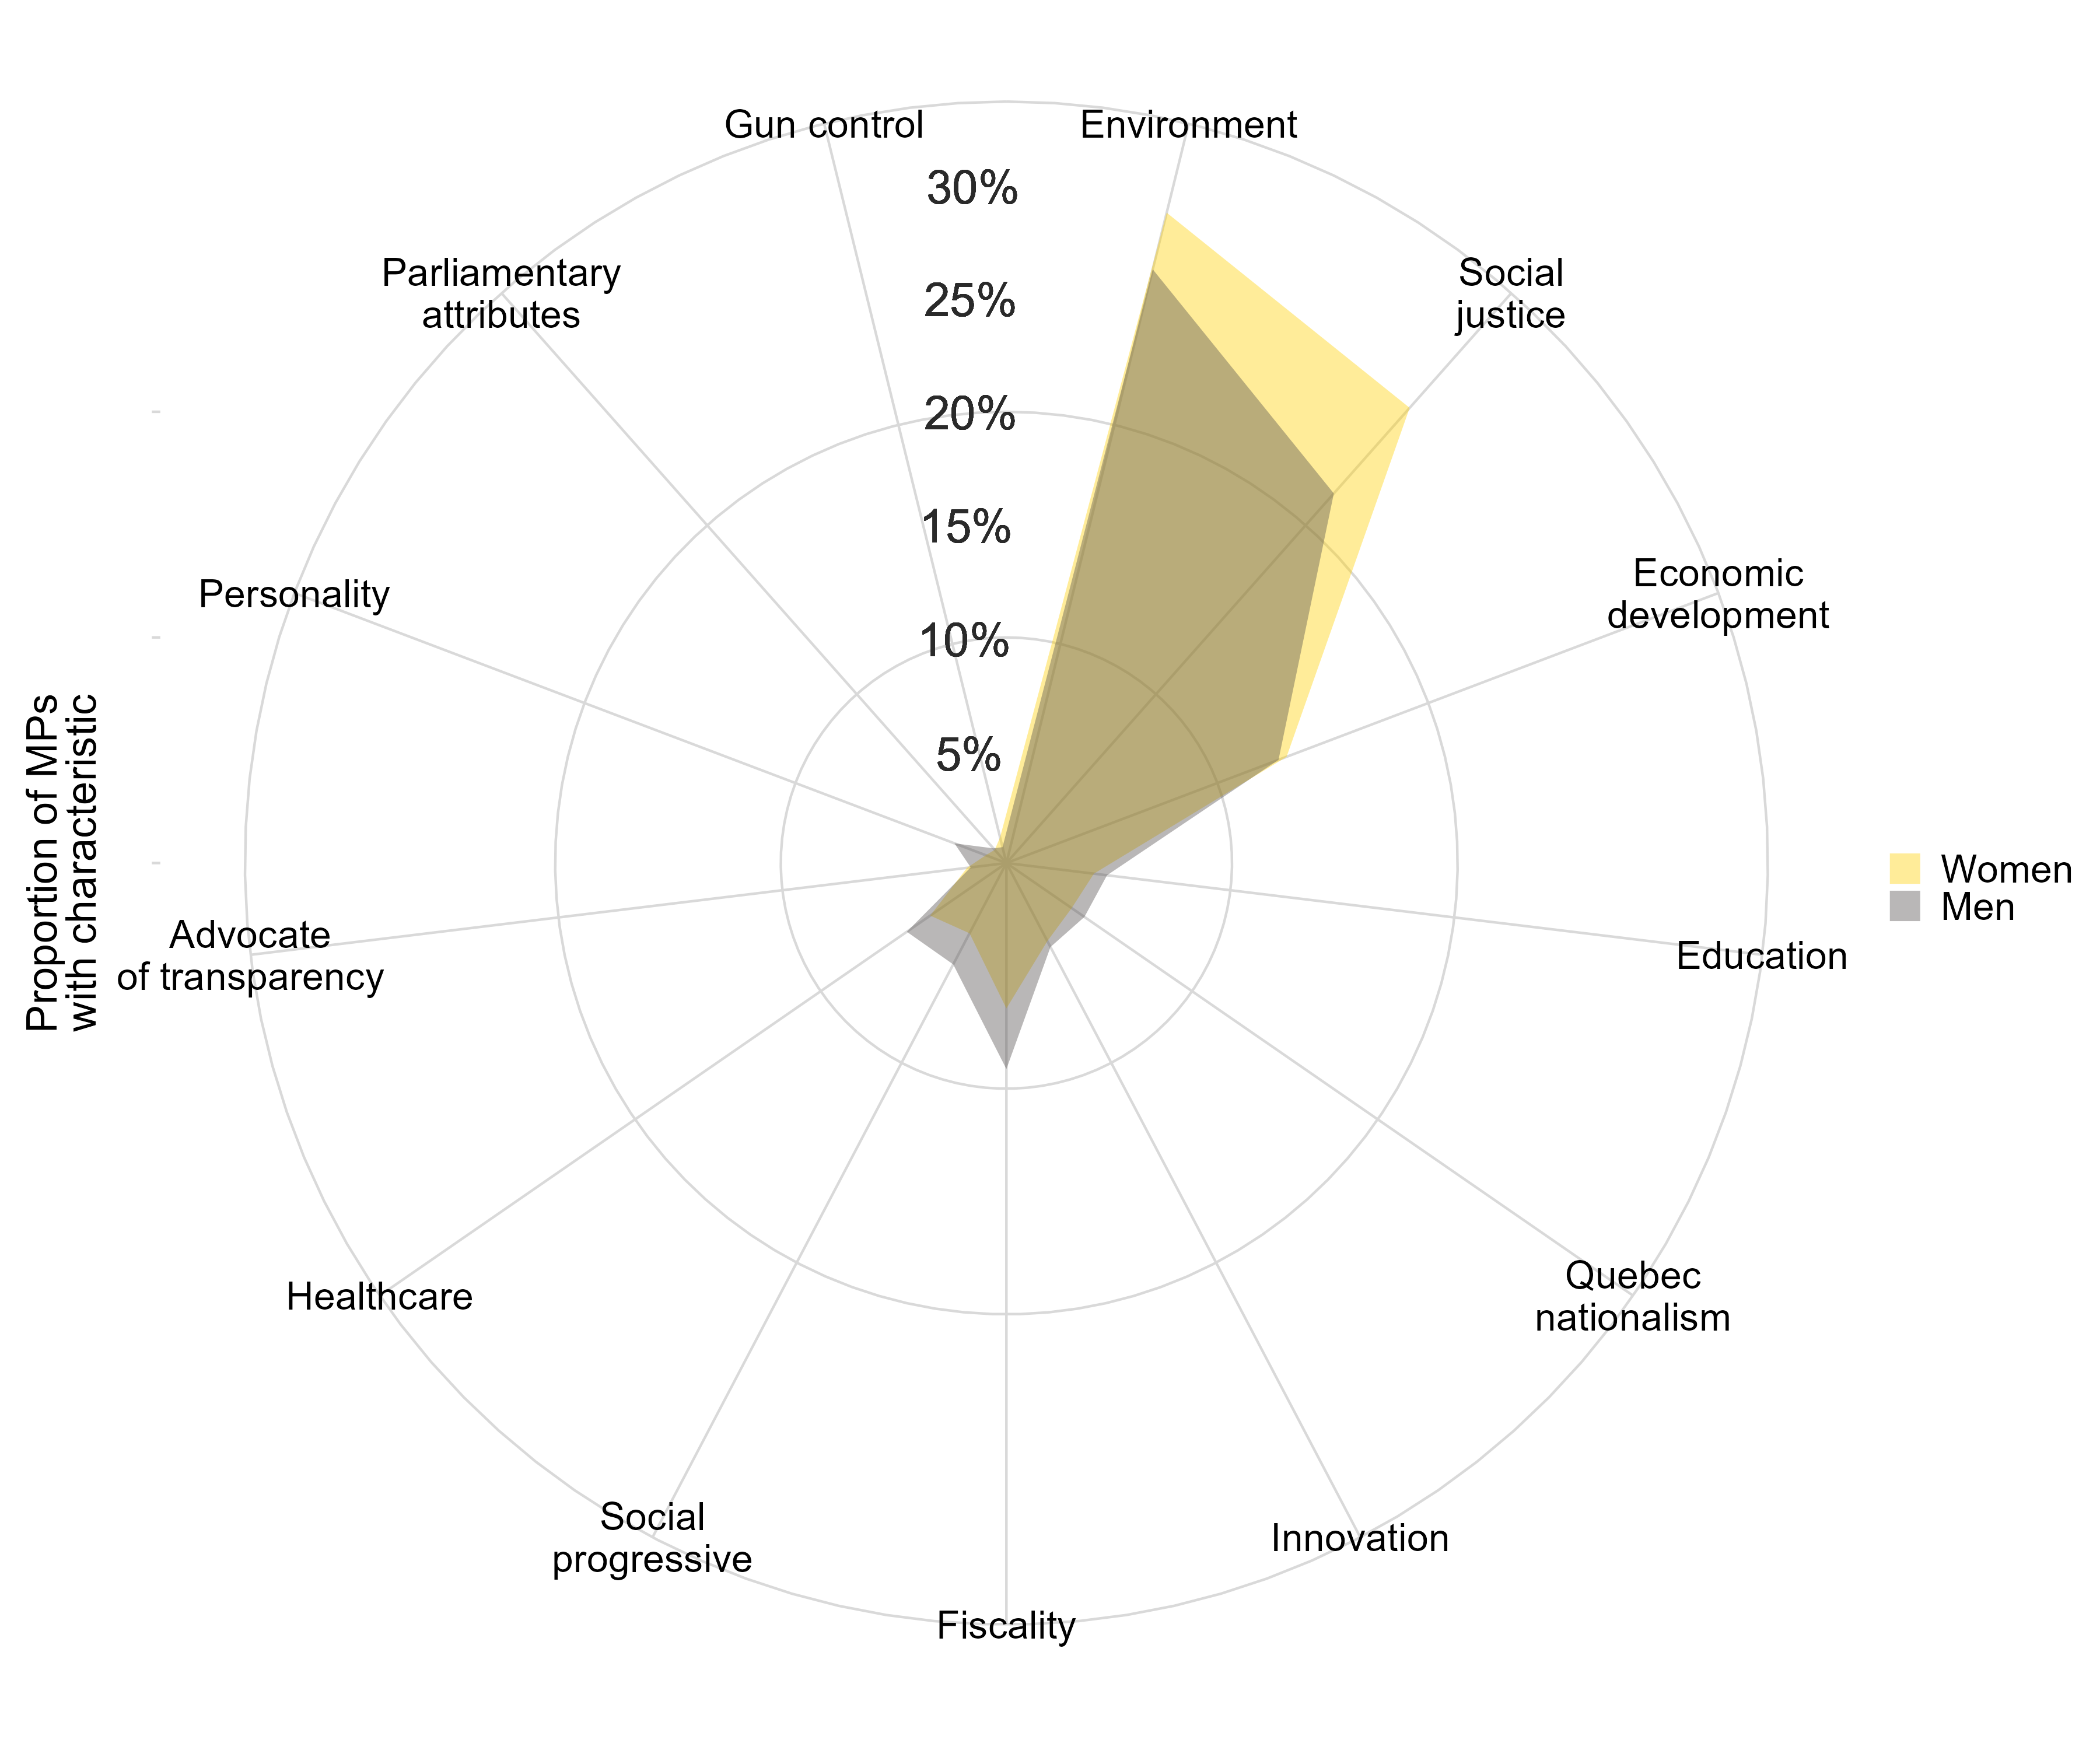
\includegraphics[width=\textwidth]{by_gender_qc.png}
        \caption{Quebec Provincial MPs}
    \end{subfigure}
    \hfill
    \begin{subfigure}[b]{0.45\textwidth}
        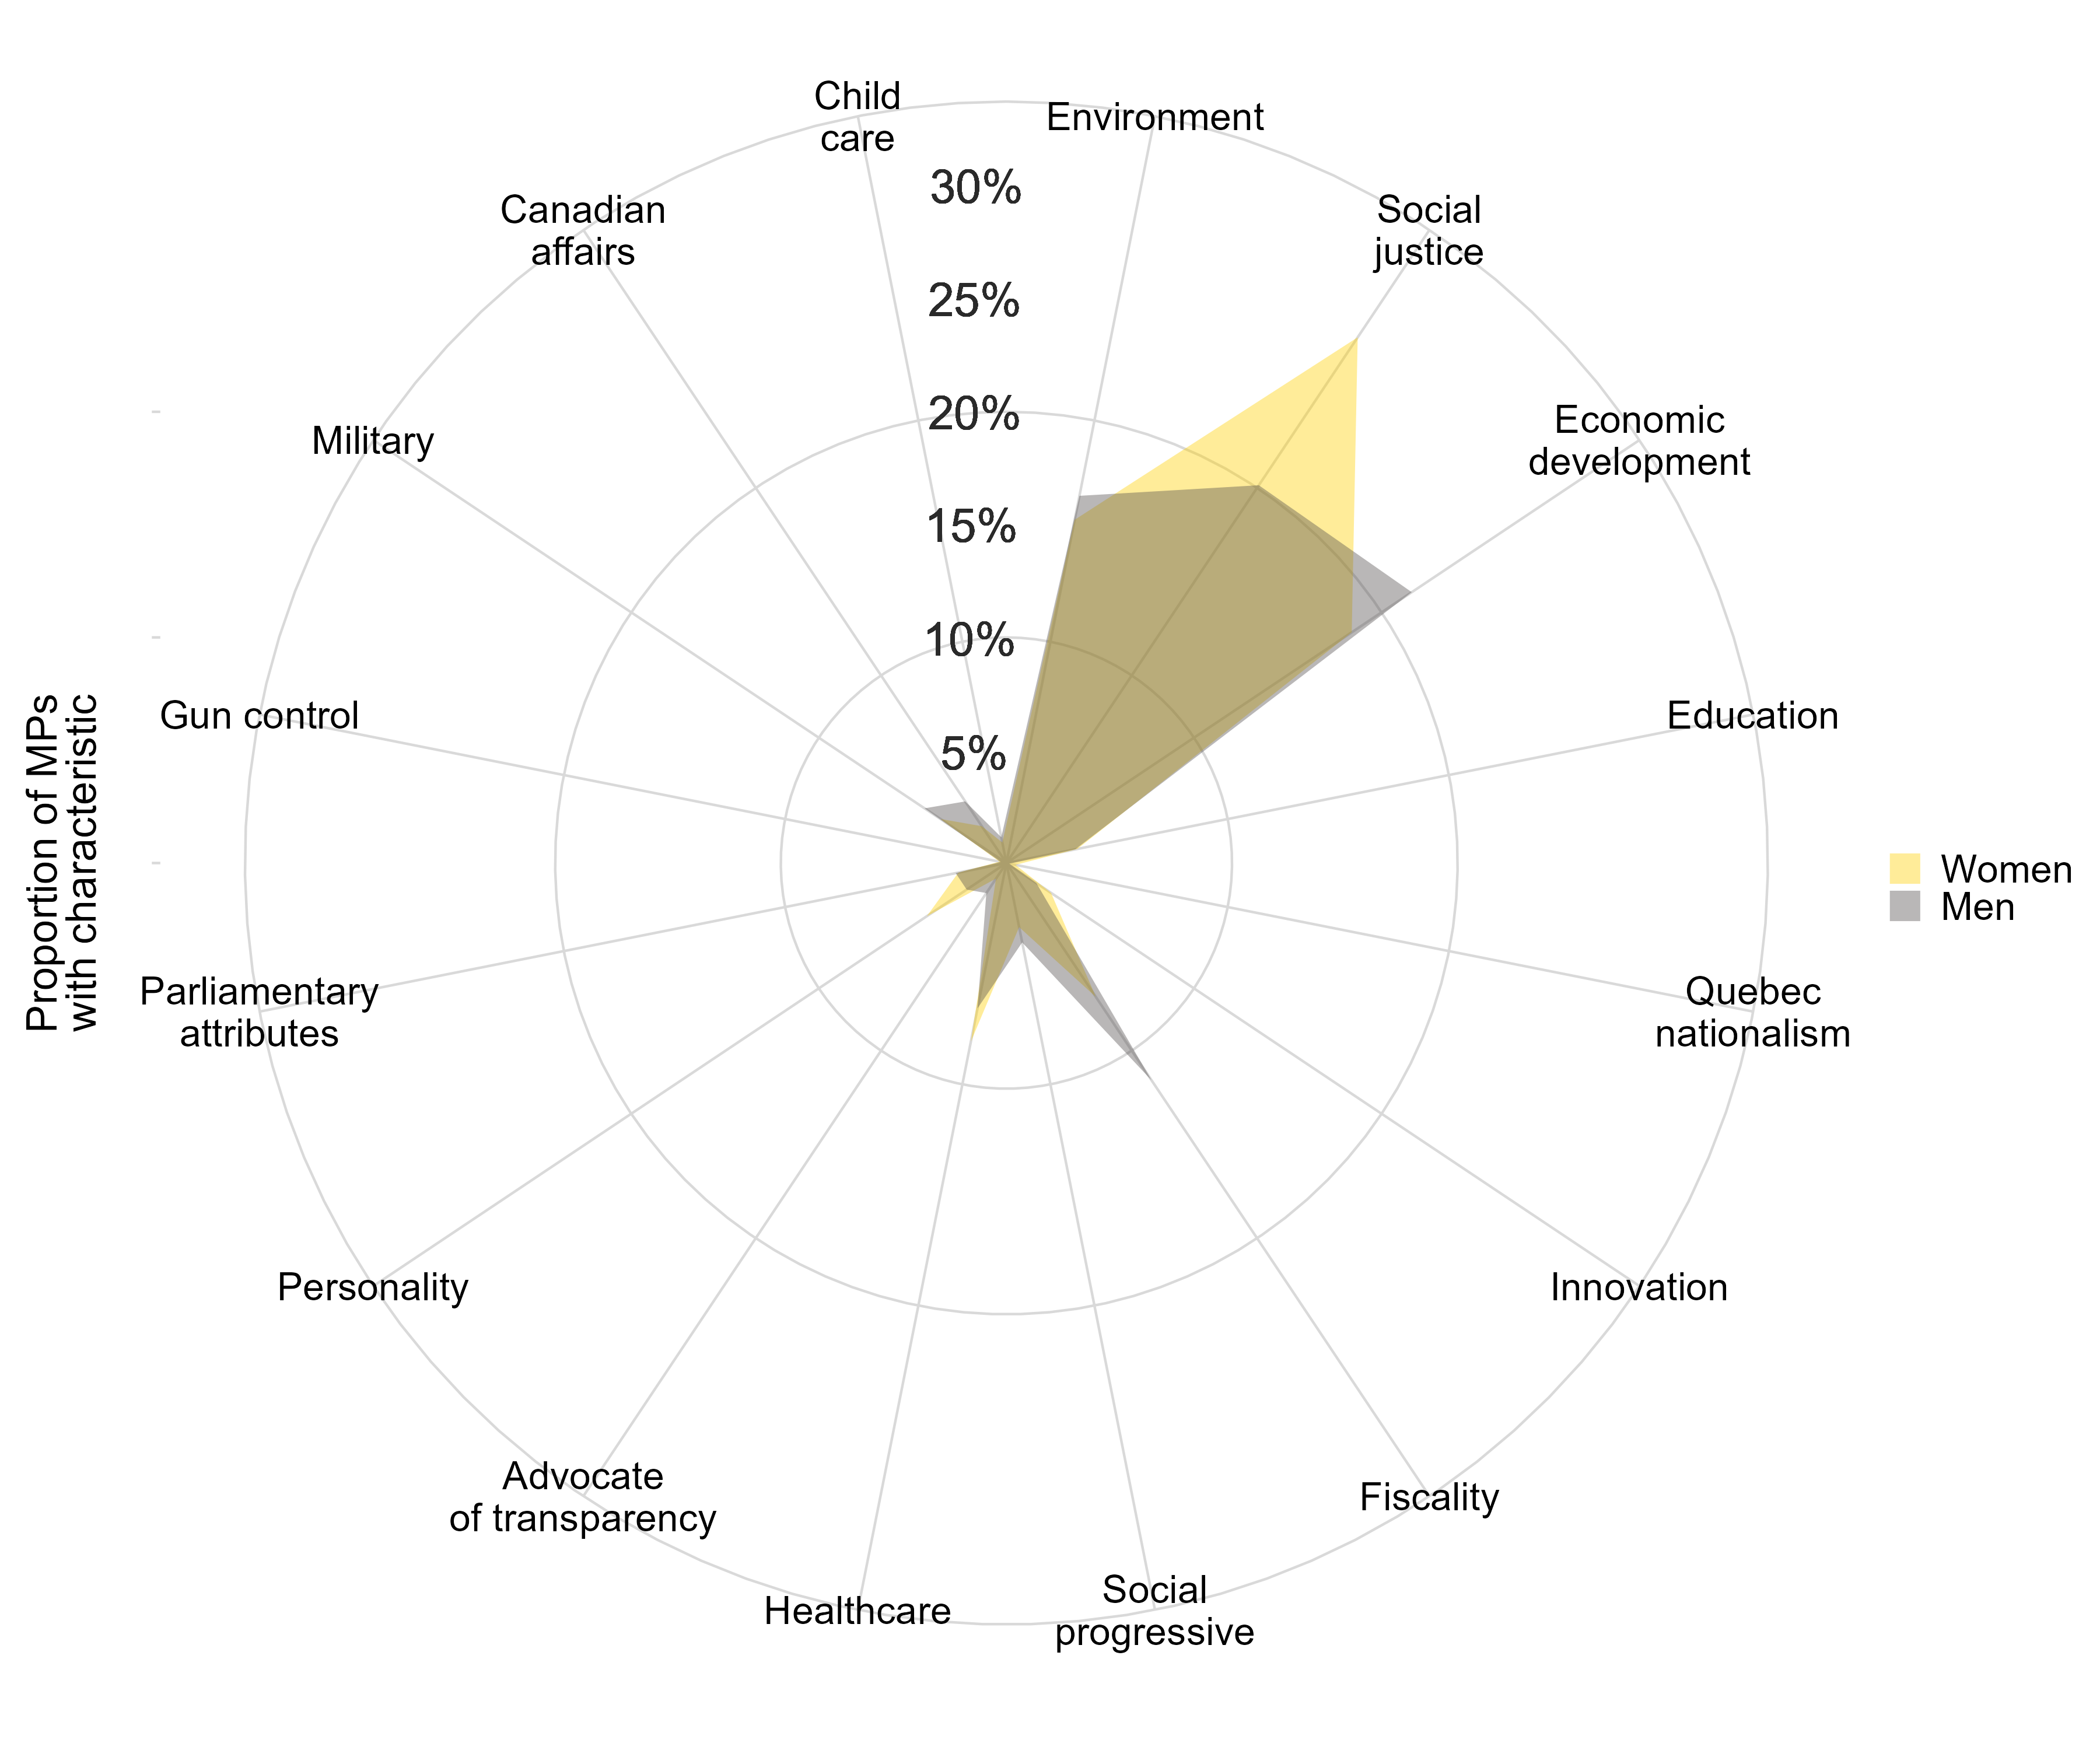
\includegraphics[width=\textwidth]{by_gender_fed.png}
        \caption{Canada federal MPs}
    \end{subfigure}

    \caption{Analysis of \textit{davinci-003} Model's Most Used Characteristic Issues by Gender}
    \begin{minipage}{0.9\textwidth}
        \footnotesize \textit{Note}: Theme labeling is derived from the Novacene AI clustering algorithm.
    \end{minipage}
    \label{bygender}
\end{figure}

\textit{Figure \ref{bygender}} shows the proportional distribution of the themes used by ChatGPT for each gender. For federal MPs, it is interesting to observe that ChatGPT mobilizes the theme of \textit{social justice} at a proportion of 28.02\% for women compared to 20.14\% for men. ChatGPT also uses the theme of \textit{economic development} more often for men (21.61\%) than for women (18.41\%). Another discrepancy observed in our dataset between men and women at the federal level is in the distribution of use of the \textit{fiscality} theme. ChatGPT used this theme at a rate of 11.58\% for men and 7.14\% for women. \par
At the provincial level, the main differences between men and women were most striking with themes concerning the \textit{environment}, \textit{social justice}, and \textit{fiscality}.

\subsubsection{Comparing Quebec and Canada}

\begin{figure}[H]
\centering
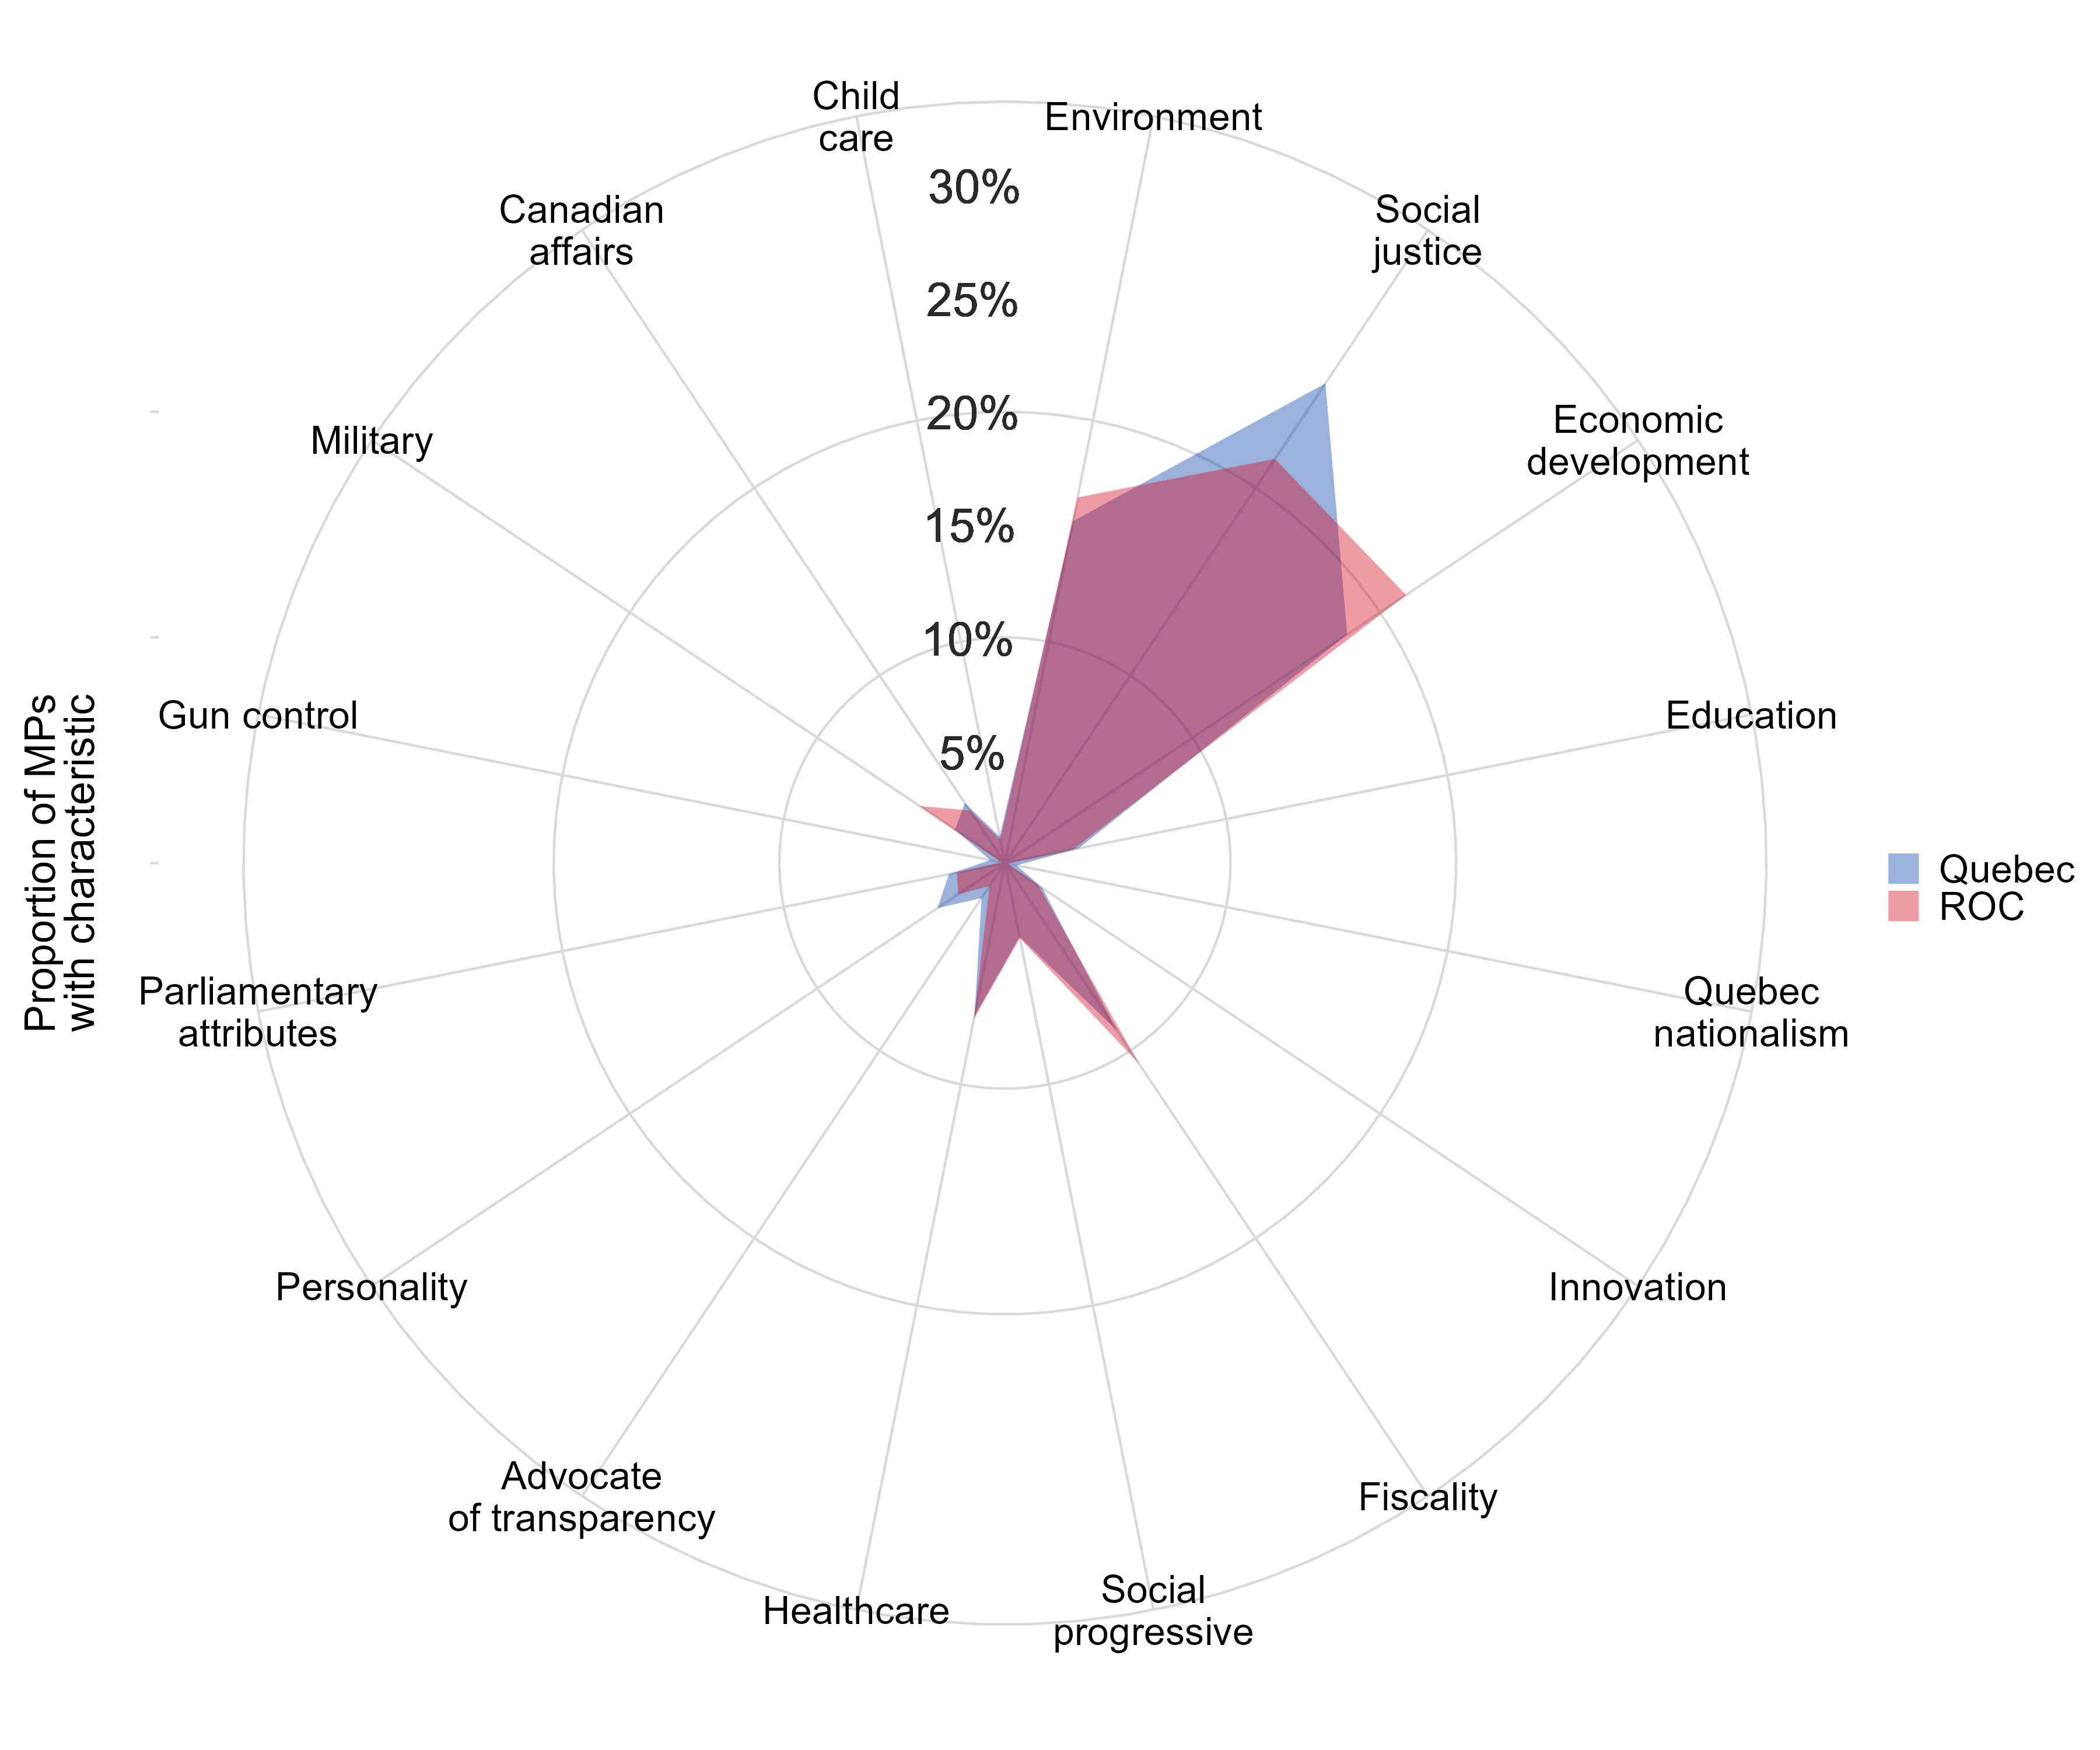
\includegraphics[scale=0.5]{by_qc_roc.png}
\caption{Comparison of the characteristics most used by \textit{davinci-003} Model's to describe Quebec versus Canadian MPs}
\begin{minipage}{0.7\textwidth}
\footnotesize \textit{Note}: Theme labeling is derived from the Novacene AI clustering algorithm.
\end{minipage}
\label{byqcroc}
\end{figure}

\textit{Figure \ref{byqcroc}} illustrates the differences in the use of main themes between federal-level MPs from Quebec and MPs from the rest of Canada. The principal differences observed concern the themes of \textit{social justice} and \textit{economic development}. The proportion of the \textit{social justice} theme was 25.57\% for federal MPs from Quebec and 21.54\% for federal MPs from the rest of Canada. We also note a proportion of the \textit{economic development} theme of 18.24\% for federal MPs from Quebec and 21.38\% for federal MPs from the rest of Canada. The relative scarcity of \textit{Quebec nationalism} theme is also surprising. The absence of a considerable difference between MPs from Quebec and the rest of Canada is also to be noted.



\section{Discussion}
In light of the increasing popularity of ChatGPT and its apparent potential for continued growth and widespread usage, and while the goal of this shorter note is not to provide a meaningful measure of algorithmic biases as others do \parencite{hartmann_etal23, santurkar_etal23, rutinowski_etal23, kim_lee23}, it sets out to present a new type of dataset that should be of great interest to political science researchers. By using the OpenAI API and combining it with other data sources, we created and shared a dataset that can be used for multiple purposes such as testing the potential biases of ChatGPT in the political context of an election. As was highlighted by the cited literature in this article, accessible LLMs like ChatGPT could become heuristic tools such as VAAs during election campaigns in the near future. Given the influence of these types of applications on vote turnout and vote decisions, it is crucial for political scientists to understand and explain their potential biases to ensure the integrity of democratic processes. This dataset (and the way it was collected) provides a starting point for achieving this.
The descriptive statistics presented in this article reveal some light discrepancies in how OpenAI's model perceives each political party, distinguishes between men and women, and differentiates Quebec MPs from other Canadian MPs. Whether these discrepancies represent actual biases and, if so, whether they stem from the model's training corpus, its parameters, or human-made boundary setting, remains a subject to be foraged into by future researchers.\\
Continuing along this line of thinking, a lot of research designs offer the potential for further exploration of this question using datasets such as the one presented in this note. In the first place, this dataset could be cross-referenced with human-generated data such as parliamentary speeches, survey data, tweets, Wikipedia articles, etc. A comparison with these other data sources could generate various hypotheses on the nature of ChatGPT's biases. Another interesting research avenue would be to take into account the order in which OpenAI's model returned the different characteristics (available in the provided dataset). Giving more weight to the first characteristics provided by the model could potentially add more variance between parties, genders, and regions. The study of AI and LLMs in the context of political science is novel and the research potential is large. Understanding how data can be retrieved and analyzed is critical. It should be encouraged to dig deeper into this topic.

\newpage
\printbibliography


\appendix

\newpage
\section{Snippet of code to prompt \textit{davinci-003}}
\label{appendix:codesnippet}

The following Python code snippet was used to prompt \textit{davinci-003} about Quebec's provincial MPs. This code snippet assumes the user has correctly set up its OpenAI API key and installed the necessary packages. For more detailed information about these particular steps, see the Github repository linked to this article.

\begin{minted}[frame=lines,framesep=2mm,baselinestretch=1.2,bgcolor=white,linenos,tabsize=2,breaklines]{python}
# Choosing an OpenAI model
model_engine = "text-davinci-003"
# Model parameters
parameters = {
    "temperature": 1.0,
    "max_tokens": 1000,
    "top_p": 1,
    "frequency_penalty": 0,
    "presence_penalty": 0,
}

# Generate an empty dataframe to save output during the loop
df_output = pd.DataFrame(columns=["mp_id", "name", "characteristics"])

## Create a prompt_template. [INSERT_NAME] will be replaced by MPs' names in the loop
prompt_template = "Provide a list of 10 key characteristics describing Quebec MP [INSERT_NAME]'s policies formated in a .csv style output, all on the same line. (ex: MP name, Characteristic 1, characteristic 2, characteristic 3, characteristic4, characteristic 5, characteristic 6, characteristic 7, characteristic 8, characteristic 9, characteristic 10)"

# Create a loop for each mp
for i in range(len(mp_ids)):
    # id and name of MP at this stage in the loop
    mp_idi = mp_ids[i]
    namei = names[i]
    
    # Clear the content of df_output
    df_output.drop(df_output.index, inplace=True)

    # Replace [INSERT_NAME] by namei (the current MP's name in the loop)
    prompt = prompt_template.replace("[INSERT_NAME]", namei)

    
    try:
    # Prompt OpenAI model
        response = openai.Completion.create(engine=model_engine, prompt=prompt, **parameters)
        generated_text = response.choices[0].text.strip()

        # Concatenate OpenAI model's response into df_output
        df_output = pd.concat([df_output, pd.DataFrame({"mp_id": [mp_idi], "name": [namei],
        "characteristics": [generated_text]})], ignore_index=True)

        # Append DataFrame to CSV starting from row 2
        if i == 0:
            # Write header for the first iteration
            df_output.to_csv(output_filename, mode='a', index=False)
        else:
            # Skip header starting from the second iteration
            df_output.to_csv(output_filename, mode='a', index=False, header=False)

        print(df_output)
    except Exception as e:
        print("error at mp_id" + mp_idi + "-" + namei)
\end{minted}
\end{document}






